\chapter{Modelling of 2 GW, 66 kV HVAC Offshore Network with MMC-HVDC Transmission}\label{4}
This chapter details the development of a multi-gigawatt (focus of 2 GW), 66 kV \gls{HVAC} network connected to a Modular Multi-level Converter (\gls{MMC}) offshore converter station. Like in Chapter \ref{3}, an average \gls{EMT} modelling depth is used (i.e. focus on the study of three-phase faults occurring in a balanced system), and the model and simulations are conducted in RSCAD. The model depicts the connection of several \gls{OWF}s through a 66 kV \gls{HVAC} offshore network contributing a total of 2 GW installed capacity. The power is transferred to the onshore system through \gls{MMC} based \gls{HVDC} links. The focus is to investigate the dynamic performance of such a system when subjected to severe disturbances (e.g. three-phase line to ground fault) in the \gls{AC} part of the network. The action of both the Direct Voltage Control (\gls{DVC}) in \gls{WG}s and the voltage control in \gls{MMC} is examined in detail to understand the voltage performance and the power flow distribution based on simulations performed in RSCAD. %Firstly, the topology selected for the network is explained, and then the large scale network layout with all the components is detailed. The control structures utilized in the network is described in the final part of this chapter.

\section{Assumptions and definition of the topology for the 2 GW Offshore Network}
The initial aspect that needs to be considered for a 2 GW system is the topology of the network. The popularity of \gls{MMC} due to its improved controllability and superior system performances has lead way for the increasing demand for \gls{MMC}-\gls{HVDC} transmission for integration of long distance \gls{OWF}s. For the connection of new \gls{OWF}s in the vicinity of the already existing ones, parallel operation of \gls{MMC}-\gls{HVDC} transmission systems can be expected in the near future with multiple connections to the onshore system. Such type of schemes increase the interest in hybrid systems with the "hub-and-spoke" principle proposed by ABB \cite{abb_hvdc_2018} and represented in Figure \ref{fig:ABB_Hub_Spoke_3}. Figure \ref{fig:ABB_Hub_Spoke_3}a) represents the connection of multiple \gls{OWF}s to the offshore converter station, and power is transferred to the onshore system through multiple \gls{HVDC} links. Such a layout provides redundancy in the network by supplying offshore wind power to at least one onshore system if one of the \gls{HVDC} links gets disconnected. The system operability is also improved at the time of disturbances in one of the onshore \gls{AC} networks \cite{lescale2012parallelling}. A stage-wise construction of such a \gls{HVDC} network is easier to be achieved by the developers \cite{irnawan2019planning}. Another layout involves the \gls{OWF}s to transfer power to the onshore system through a single \gls{MMC} unit with multi-terminal \gls{HVDC} connections as shown in Figure \ref{fig:ABB_Hub_Spoke_3}b). However, in such a layout, the idea of scaling of offshore wind power is limited to the installed capacity of the \gls{MMC} unit. Lastly, the \gls{OWF}s can be connected through \gls{AC} links to a back-to-back \gls{HVDC} converter station as shown in Figure \ref{fig:ABB_Hub_Spoke_3}c). Long distance \gls{HVAC} transmission is required in this case, for the transfer of power from \gls{OWF}s to the onshore network and contribute to high losses in the network when compared to \gls{HVDC} transmission for larger distances.

The idea in this section is to expand the single \gls{OWF} model network in Figure \ref{fig:WT1_Model_RSCAD} for a 2 GW offshore wind power. This could be made possible by connecting four such \gls{OWF} models in parallel with each generating 500 MW of power. On the other hand, a offshore converter station of 2 GW is required to transfer this generated amount of power to the onshore system. However, the currently deployed (state-of-the-art) \gls{MMC}-\gls{HVDC} transmission, has a maximum rated capacity of 1200 MW \cite{cigre2005b4}. Hence, with the available technology, two \gls{MMC} units will be required for 2 GW of power transmission. Taking the aforementioned factors into account, a layout similar to the Figure \ref{fig:ABB_Hub_Spoke_3}a) is developed for this work and is depicted in Figure \ref{fig:WT4_MMC2}. 

\begin{figure}[H]
\centering
%\hspace*{-1.2cm}
    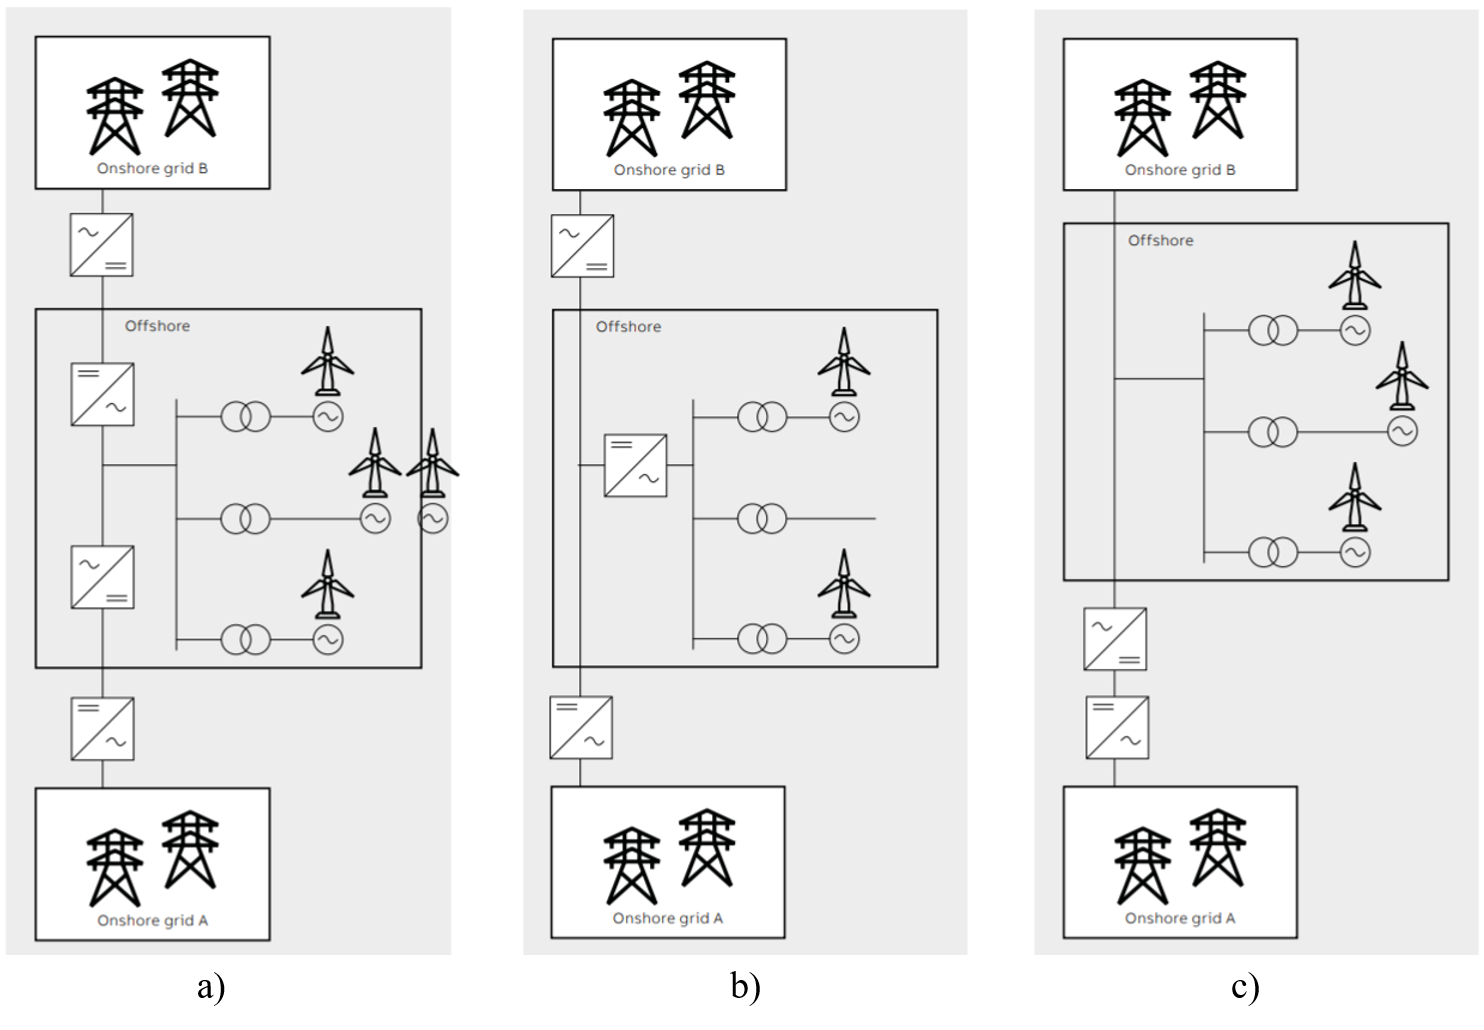
\includegraphics[height = 10cm,width = 15cm]{Diagrams/Chapter_4/ABB_Hub_Spoke_3.png}
    \caption{a) Hub-and-spoke with multiple HVDC links b) Hub-and-spoke with multi-terminal HVDC system, c) Hub-and-spke with AC links and HVDC back-to-back station \cite{abb_hvdc_2018}}
    \label{fig:ABB_Hub_Spoke_3}
\end{figure}

% Therefore by using the average \gls{EMT} model of an \gls{MMC} described in utilizing the available models for \gls{MMC}s, to enhance and understand the operation of Type-4 \gls{WG}s in parallel operation and their coordination with \gls{MMC}s, an \gls{AC} collector grid topology with parallel connection of two point-to-point \gls{HVDC} transmission system is implemented for this thesis work in RSCAD. 

\subsection{Processors in RSCAD}\label{split_system}
The simulations in RSCAD can be run in either NovaCor or PB5 processor cards. NovaCor processor is used for this work as they have 2-3 times the simulation capacity of a completely loaded PB5 processor \cite{noauthor_novacor_nodate}. For an extensive power system network, NovaCor processor requires a part of the system to be placed in a separate subsystem. RSCAD allows provision for splitting of the network into subsystems if the network is large. The splitting is done by right-clicking on the main subsystem tag and choosing "Add Subsystem" as shown in Figure \ref{fig:subsystem_RSCAD} and this feature is utilized in this section. Tline modules are used to connect between subsystems. The process is explained in Section \ref{Tline_cable_RSCAD} in detail.

There are two NovaCor processors available in TU Delft and they are equipped with four cores each. These cores are utilized to solve the overall network solution, auxiliary components (such as transformers, cables, generators etc.) and the controls present in the simulation. Assignment of cores for solving various components of the network is an important step that needs to be considered while modelling, as they depict the total load that is distributed over the available cores. The process is detailed in Section \ref{Aggregated_OWF_large_scale}. 

\begin{figure}[H]
\centering
%\hspace*{-1.2cm}
    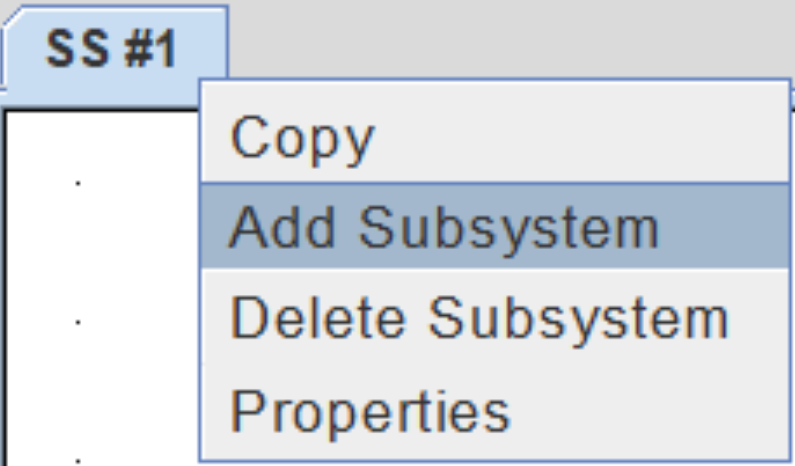
\includegraphics[height = 2cm,width = 3.5cm]{Diagrams/Chapter_3/Subsystem.PNG}
    \caption{Adding subsystems in RSCAD}
    \label{fig:subsystem_RSCAD}
\end{figure}

\begin{figure}[H]
\centering
%\hspace*{-1.5cm}
    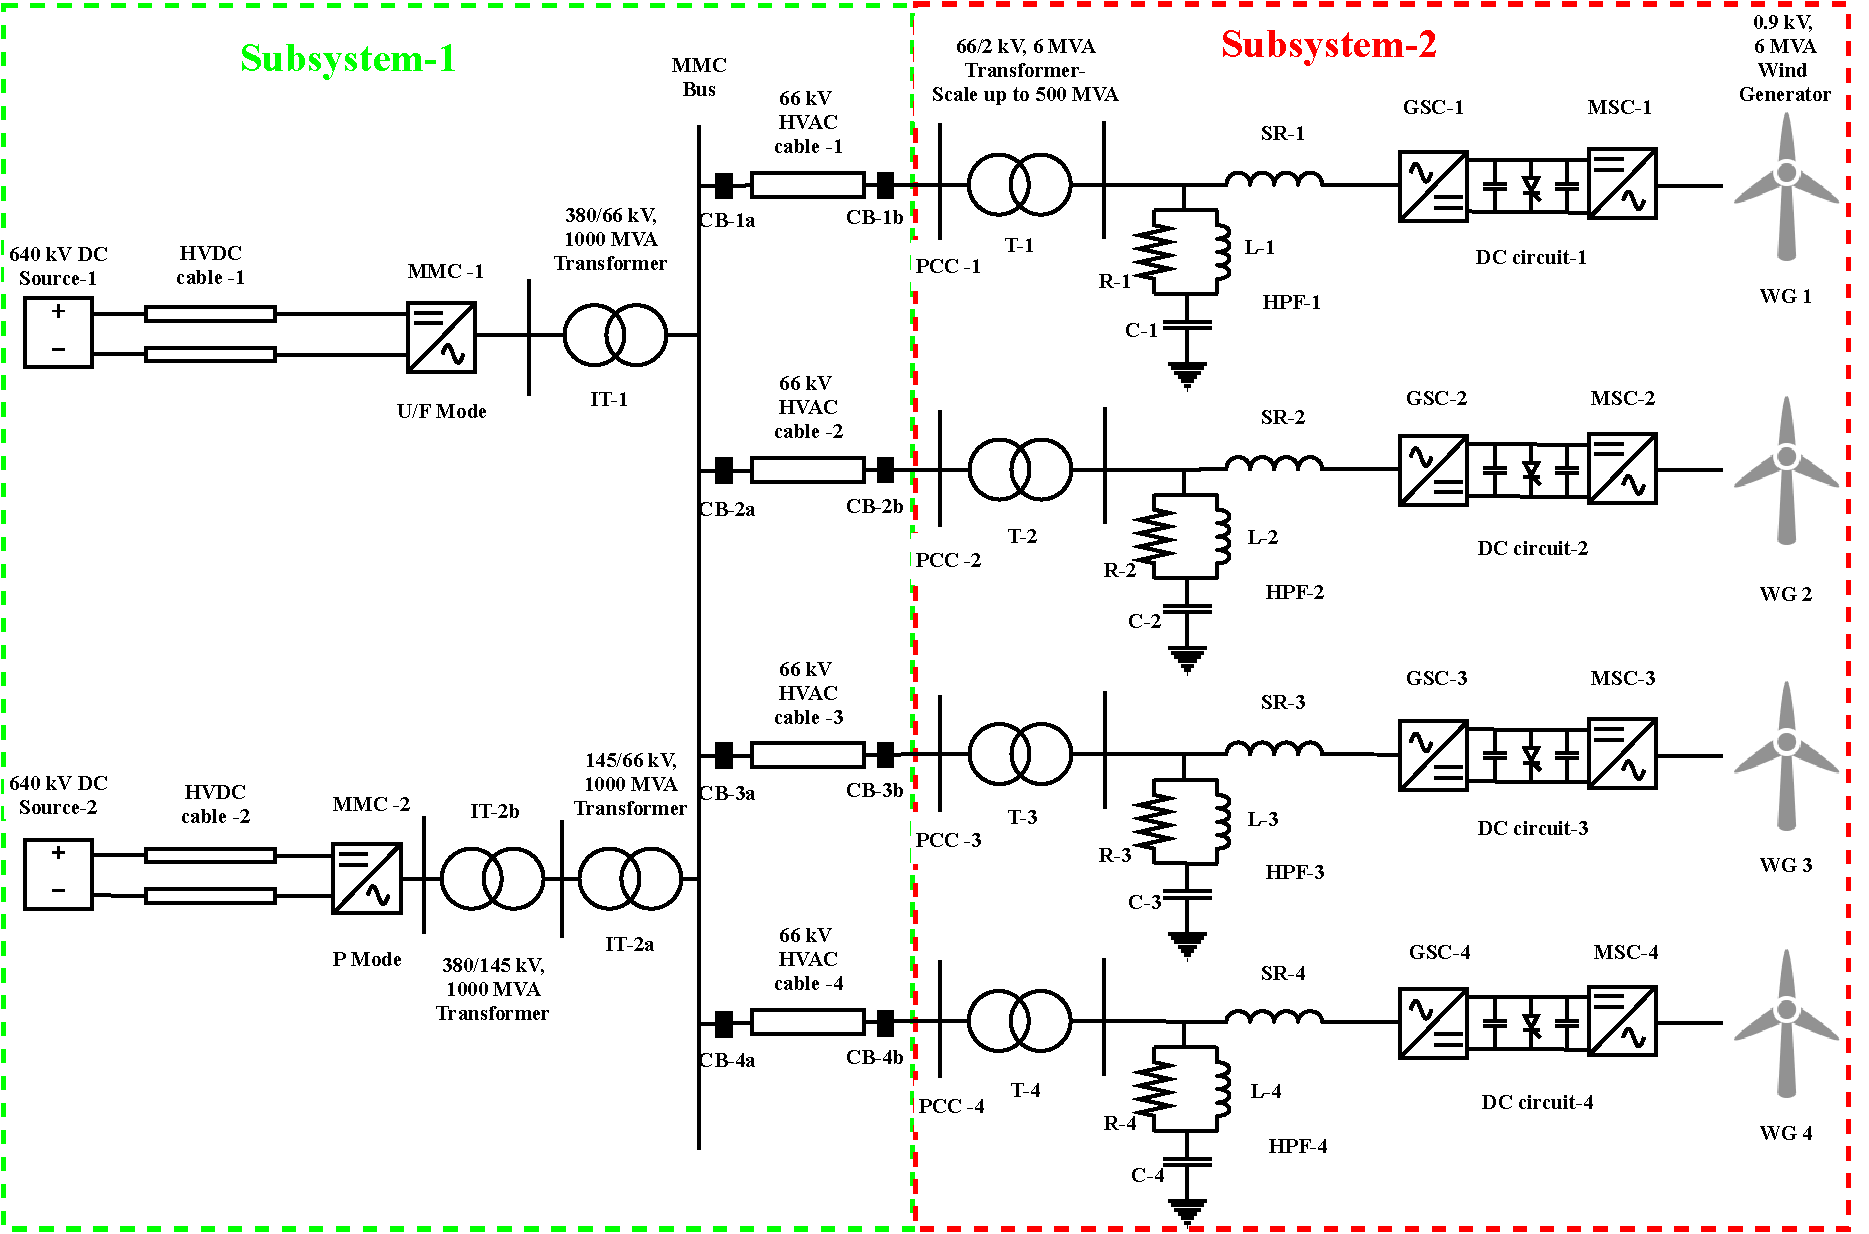
\includegraphics[height = 12.5cm,width = 17cm]{Diagrams/Chapter_4/WT4_MMC2_new.pdf}
    \caption{Single line diagram of 2 GW, 66 kV HVAC offshore network connected to 2 x 1 GW HVDC links with offshore MMC stations in RSCAD}
    \label{fig:WT4_MMC2}
\end{figure}



\section{Layout of 66 kV HVAC 2 GW Offshore Network in RSCAD}
The development of the layout involved three steps:


of the model is developed by connecting four \gls{OWF} A modular approach is considered to implement the connection of four \gls{OWF}s. The aggregated representation of a \gls{OWF} implemented in Section \ref{WT1_ACsource_RSCAD_Test_Layout} is modularized to form the large scale offshore network. The single line diagram of the network is depicted in Figure \ref{fig:WT4_MMC2} and the major components of the 66 kV \gls{HVAC} 2 GW network include :
\begin{itemize}
    \item Four aggregated \gls{OWF}s, each with 500 MW installed capacity represented by the following components:
    \begin{itemize}
        \item A single Wind Generation System with 
    \begin{itemize}
        \item Permanent Magnet Synchronous Generator (\gls{PMSG})
        \item Machine Side Converter (\gls{MSC})
        \item \gls{DC} circuit
        \item Grid Side Converter (\gls{GSC}) 
    \end{itemize}
        \item High Pass filter (\gls{HPF}) with series reactor
        \item \gls{OWF} transformer
    \end{itemize}
    \item Four \gls{HVAC} cables  
    \item Two offshore converter transformers
    \item Two \gls{MMC}s
    \item Two \gls{HVDC} cables
\end{itemize}



\subsection{Aggregated OWF}\label{Aggregated_OWF_large_scale}
The \gls{OWF} model described in Section \ref{OWF} is used here for all the four \gls{OWF}s. As the network is extensive, it is split into two subsystems in RSCAD as shown in Figure \ref{fig:WT4_MMC2} by employing the technique explained in Section \ref{split_system}. The four \gls{OWF}s are modelled in subsystem 2 and the rest of the system is modelled in subsystem 1. Each subsystem requires one rack for operation and hence two NovaCor racks are used for the network simulation. It is also possible to simulate the network with PB5 processor. However, this requires a total of three subsystems since PB5 racks allow only small network solutions to be solved in one rack \cite{noauthor_pb5_nodate}. Therefore, two \gls{OWF}s are to be modelled in subsystem 3, other two \gls{OWF}s in subsystem 2 and the rest of the network in subsystem 1. Hence this would require a total of three PB5 racks. However, the simulations are considered only in NovaCor processed for this study.  


Since there need to be four different small-time step blocks representing four \gls{OWF}s, each block needs to be set with different step sizes so as to avoid conflict during initialization. These step sizes are only used for initialization and the actual step sizes can be viewed in the "Map File" as mentioned in Section \ref{OWF}. Moreover, if the time-steps are not initialized properly, it could lead to the occurrence of a time-step overflow error during run time. Another important parameter to be considered here is the assignment of the cores for the small-time step boxes. 

As mentioned in Section \ref{split_system}, cores are responsible for solving the entire network solution. NovaCor processor has four cores and each component used in the network can be assigned to specific cores (1 to 4 in number). The cores can be assigned manually or can be done automatically (why u did manually). The core allocation of the small-time step boxes representing \gls{OWF}s in this network is as shown in Table \ref{tab:Core_assignment_sub2}.  

   

\begin{table}[H]
\centering
\begin{tabular}{|c|c|}
\hline
\textbf{Small time-step block} & \textbf{Core assignment} \\ \hline
OWF-1                          & 4                        \\ \hline
OWF-2                          & 1                        \\ \hline
OWF-3                          & 3                        \\ \hline
OWF-4                          & 1                        \\ \hline
\end{tabular}
\caption{Core assignment of OWF models in subsystem 2}
\label{tab:Core_assignment_sub2}
\end{table}

\subsection{HVAC Cables}\label{Tline_cable_RSCAD}
 The \gls{HVAC} cables transfer power from the \gls{OWF}s in subsystem 2 to the \gls{MMC} bus in subsystem 1 as can be seen in Figure \ref{fig:WT4_MMC2}. The cables are rated at 66 kV and are of length 30 kms. In RSCAD, subsystems can be connected using the Tline module available in the RSCAD modules section as denoted by a red box in Figure \ref{fig:TlineModule_mark}. This module is similar to the Cable module explained in Section \ref{HVAC_cable_RSCAD}, however Cable module does not provide the provision for splitting the network into subsystems. The Tline module can be modelled as overhead transmission line or cable. Since an offshore network modelling is considered in this work, it represents a subsea cable model. The cables here are modelled as Bergeron models with RLC data parameters (Why Bergeron). 
 
 \begin{figure}[H]
\centering
%\hspace*{-1.2cm}
    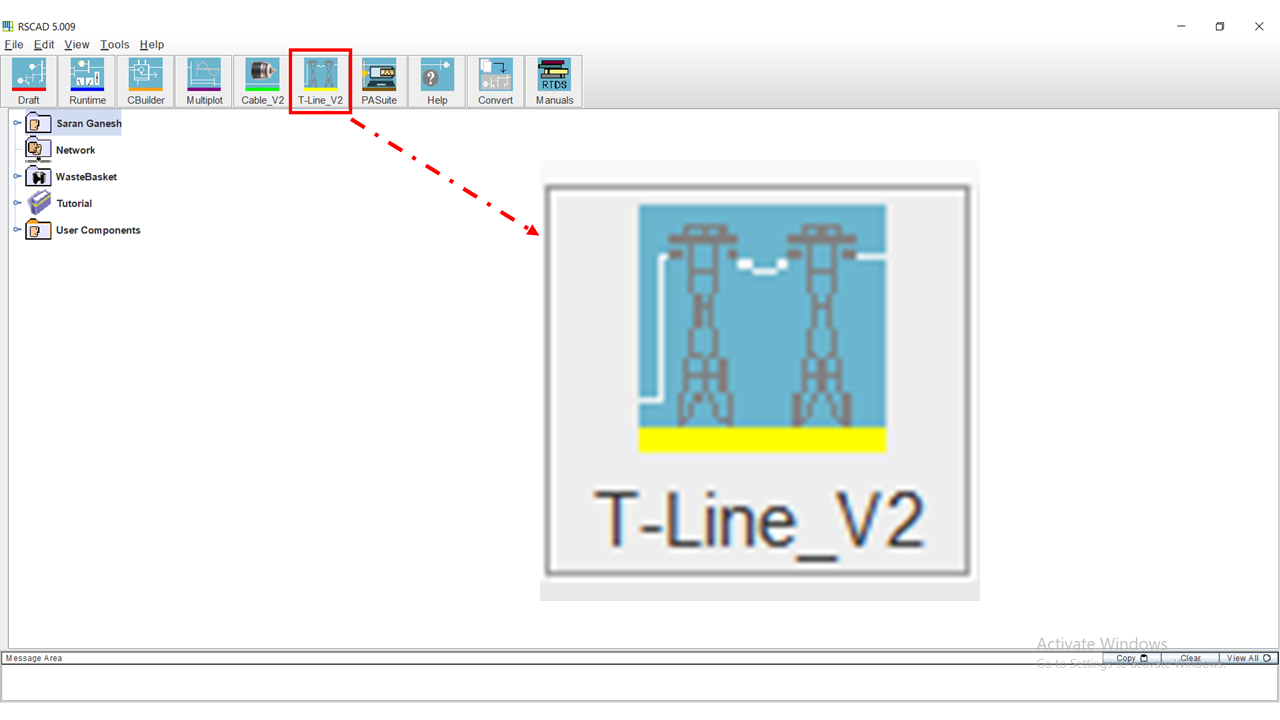
\includegraphics[height = 4.5cm,width = 7.5cm]{Diagrams/Chapter_4/Tline_module_Final.png}
    \caption{Tline module in RSCAD}
    \label{fig:TlineModule_mark}
\end{figure}
 
 In the Draft module, the cable model is added in the circuit using the unified Tline model shown in Figure \ref{fig:Tline_calculationbox_RSCAD} available in RSCAD library. The unified model consists of the following components: 
%\setlist{nolistsep}
    \begin{itemize}[noitemsep]
    \item Calculation Box
    \item Sending End Terminal
    \item Receiving End Terminal
\end{itemize}

The detailed representation of the cable parameters in Tline module, and the representation of the cable model using the calculation box, sending end terminal and receiving end terminals in the Draft module is shown in Appendix \ref{config_Tline}.

\begin{figure}[H]
  \centering
  % include first image
  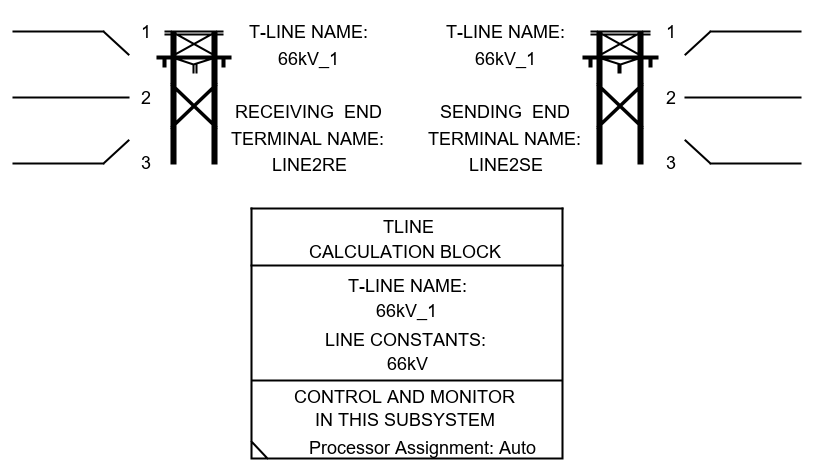
\includegraphics[height = 4.5cm,width = 7.5cm]{Diagrams/Chapter_4/TlineParaBlock.PNG}  
  \caption{Tline configuration}
  \label{fig:Tline_calculationbox_RSCAD}
\end{figure}

As the significant goal is to estimate the dynamic performance of the network under severe disturbances, a short circuit event in the middle of any \gls{HVAC} cable is tested upon. For this work, the short circuit event is modelled in the middle of HVAC cable-1. To perform a short circuit event in the middle of a 30 km long \gls{HVAC} cable in RSCAD, two cable models of 15 kms length are modelled and connected in series as shown in Figure \ref{fig:Subsystem_Trial}. The three-phase fault logic available in RSCAD library is modelled in the middle of the two cables as shown in Figure \ref{fig:Subsystem_Trial}. Both the cable models contain one set of sending and receiving end terminals. In order to connect two subsystems, the sending end terminal from the \gls{OWF} is placed in subsystem 2, and its receiving end is placed in subsystem 1. %The representation of one \gls{OWF} and one set of \gls{HVAC} cable in two subsystems in RSCAD is shown in Figure  \ref{fig:Subsystem_Trial}. All \gls{OWF}s placed in subsystem 2 are connected to the rest of the system in system 1 using \gls{HVAC} cables in a similar fashion.

\begin{figure}[H]
\centering
%\hspace*{-0.8cm}
    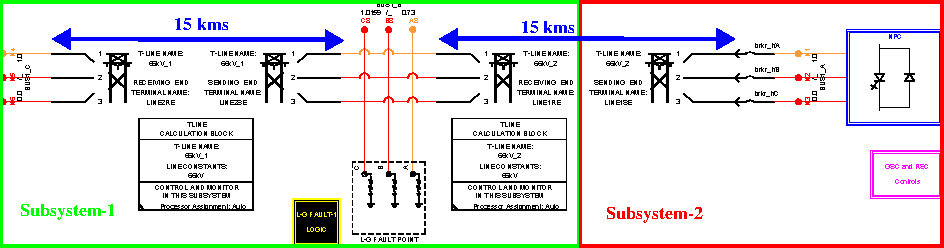
\includegraphics[height = 5.4cm,width = 17cm]{Diagrams/Chapter_4/subsystem_fault_mark.pdf}
    \caption{Representation of three-phase line to ground fault in the middle of HVAC cable-1 in RSCAD}
    \label{fig:Subsystem_Trial}
\end{figure}

\section{Offshore Converter Station}
The offshore converter station consists of the interface transformers and \gls{MMC}s. Similar to the \gls{OWF}, since many \gls{PE}s are involved in \gls{MMC} model, it is represented in a separate small time step block. Two small time step blocks are required for the representation of two \gls{MMC}s. Both the blocks are placed in subsystem 1. These two blocks must also be initialized with different step size to avoid the occurrence of an error during runtime. 
%RSCAD also allows modelling in substep environment that can have a time step as small as 500 ns if the circuit is simple.    

\subsection{Converter Transformers}
The converter transformers are connected to the \gls{AC} side of the \gls{MMC}s  as shown in Figure \ref{fig:WT4_MMC2}. They play a vital role in \cite{cigre2005b4}:
\begin{itemize}
    \item Providing a reactance between the offshore grid and the \gls{MMC}.
    \item Preventing the flow of zero sequence currents between the offshore grid and the \gls{MMC}.
\end{itemize} 

The offshore \gls{MMC} and the converter transformer are modelled in a small time step environment in RSCAD. The three identical single-phase transformer \gls{VSC} interface model available in the RSCAD library shown in Figure \ref{fig:InterfaceTrafo} is considered for this research. Delta-star type transformer configuration is used for the converter transformers for this work. \gls{MMC} is connected to the delta side of the transformer in order to isolate the zero sequence currents during faults. There are mainly two interface transformers used in this work. The transformers are rated 66/380 kV, 1000 MVA for the \gls{MMC}-1 branch and 145/380 kV, 1000 MVA for the \gls{MMC}-2 branch. Both the transformers have winding reactances of 18\% each which lies in the optimum range \cite{cigre2005b4}. Due to limitation of the control structure model in RSCAD, an additional transformer is required to convert from 66 kV to 145 kV in the \gls{MMC}-2 bus. To have a minimum effect on the impedance of the network, the leakage inductance value of this transformer is kept as low as possible. In a practical scenario, this can be avoided by using a 66/380 kV transformer directly. 

\begin{figure}[H]
\centering
%\hspace*{-1.2cm}
    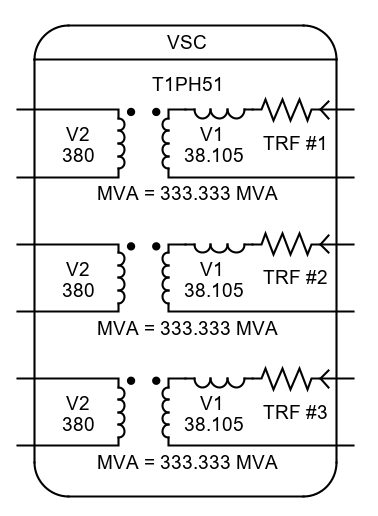
\includegraphics[height = 5cm,width = 4cm]{Diagrams/Chapter_4/InterfaceTrafo.PNG}
    \caption{VSC interface transformer model in RSCAD}
    \label{fig:InterfaceTrafo}
\end{figure}

\subsection{Modular Multilevel Converters (MMC)s}
Modular Multilevel Converters (\gls{MMC}) are the present converter topology preferred for \gls{VSC}-\gls{HVDC} transmission schemes due to their high efficiency and other advantages, as mentioned in Section \ref{HVDC_trans_theory}. They prove to be the state of the art technology for \gls{HVDC} transmission until today. RSCAD has the option of modelling the \gls{MMC} using half-bridge submodules or full-bridge submodules. Half-bridge type with 320 submodules is used for both \gls{MMC} models in this work. Both the \gls{MMC}s are connected to the \gls{DC} sources through a symmetric monopole configuration with $\pm$ 320 kV rated voltage on the \gls{DC} side and 380 kV on the \gls{AC} side. 
The \gls{MMC} model used in RSCAD internally provides capacitor voltage balancing. A Bergeron travelling wave transmission model is used to connect the \gls{MMC} in the small-time step network with the large time step network. The \gls{MMC} models considered for this research are modelled from the reference models in \cite{wachal2014guide}. \gls{DC} side of \gls{MMC}s are simplified by connecting the \gls{HVDC} cables to \gls{DC} sources since the area of study for this thesis is the \gls{AC} offshore network. 

\begin{figure}[H]
\centering
%\hspace*{-1.2cm}
    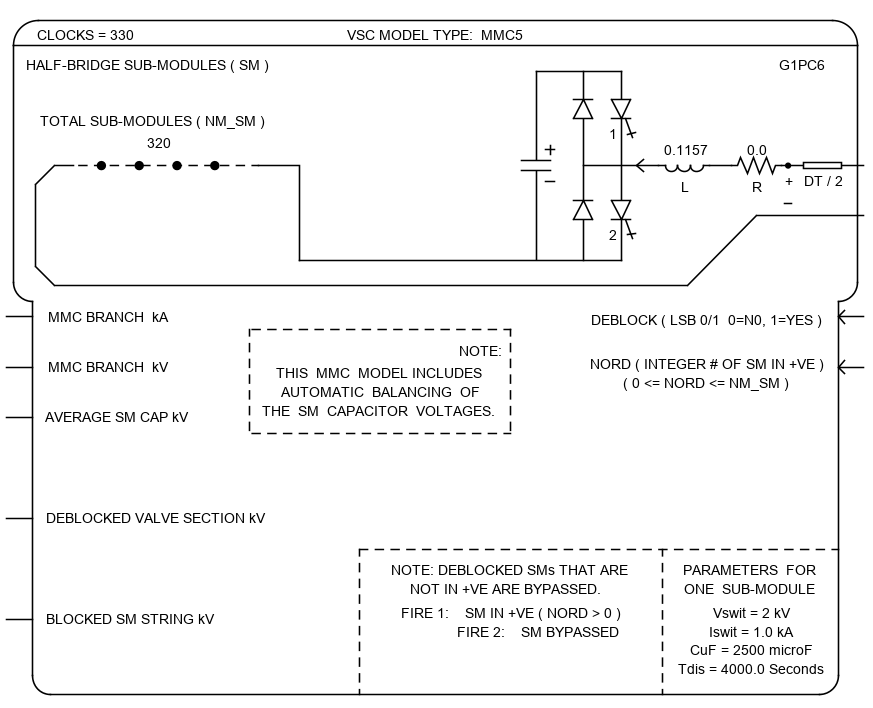
\includegraphics[height = 7cm,width = 9cm]{Diagrams/Chapter_4/MMC5_RSCAD_2.PNG}
    \caption{MMC model in RSCAD}
    \label{fig:MMC5_RSCAD_2}
\end{figure}

\section{\gls{HVDC} Cables}
The maximum voltage level for offshore projects are currently set at 600 kV, and most projects are at 525 kV \cite{lagrotteria_hvdc_2019}. The \gls{DC} voltage level for this model is chosen to be $\pm$ 320 kV. The \gls{HVDC} cables are represented in RSCAD as frequency-dependent phase domain models using the unified cable model block explained in Section \ref{HVAC_cable_RSCAD}. It is modelled in subsystem 1 connecting the \gls{MMC}s and \gls{DC} sources. 
The cable \gls{HVDC} parameters used in the RSCAD model are as mentioned in \cite{wachal2014guide}.

\section{Control structures}
This section explains the different control structures implemented and modifications made in the control scheme in converters for this work. The Direct Voltage control (\gls{DVC}) inspired from \cite{erlich_new_2017} and implemented in Section \ref{DVC_RSCAD} for Type-4 \gls{WG}s is extended for the large-scale network. There are mainly three control strategies used:
\begin{itemize}
    \item \gls{DVC} in all \gls{GSC}s
    \item Island mode control in \gls{MMC}-1
    \item Non- island mode control in \gls{MMC}-2
\end{itemize}

\subsection{DVC}
The control structure explained in Section \ref{DVC_RSCAD} is implemented for all the four \gls{WG}s. Since the same type of model is used for \gls{GSC}s in all four \gls{WG}s, the control loop parameters remain the same.

\subsection{Island mode control}
It is highly necessary to use a control strategy in any of the \gls{MMC}s which could provide the voltage and frequency reference for the \gls{MMC} bus since it is connected to a highly weak offshore network. The reference voltage is created by U/F control mode, which comes under the classification of islanded mode of control for \gls{VSC} \cite{vrana2013cigre}. For this study, the \gls{MMC}-1 is operated in the U/F mode. A basic control strategy was developed according to the illustration provided in \cite{wachal2014guide} and is shown in Figure \ref{fig:U_F_control}. This control is used for islanding mode, and hence the angle reference ($\theta$) is generated by an independent Voltage Controlled Oscillator (VCO). Such an approach provides the grid forming behaviour for \gls{MMC}-1 and is responsible for providing and absorbing power from the \gls{OWF} network as and when required. The power flow is kept in balance during the steady-state and transient condition with the help of this control.  

U/F control consists of a \gls{PI} controller which takes in error between the measured and reference \gls{PCC} voltage in p.u. and provides the reference d-axis converter voltage that is translated to abc frame as shown in Figure \ref{fig:U_F_control}. This makes the d-axis voltage to be aligned with the grid voltage and the q-axis voltage to be zero. The parameters for the proportional and integral gains used for this control are specified in Table \ref{tab:U_F_para}. 

\begin{figure}[H]
\centering
%\hspace*{-1.2cm}
    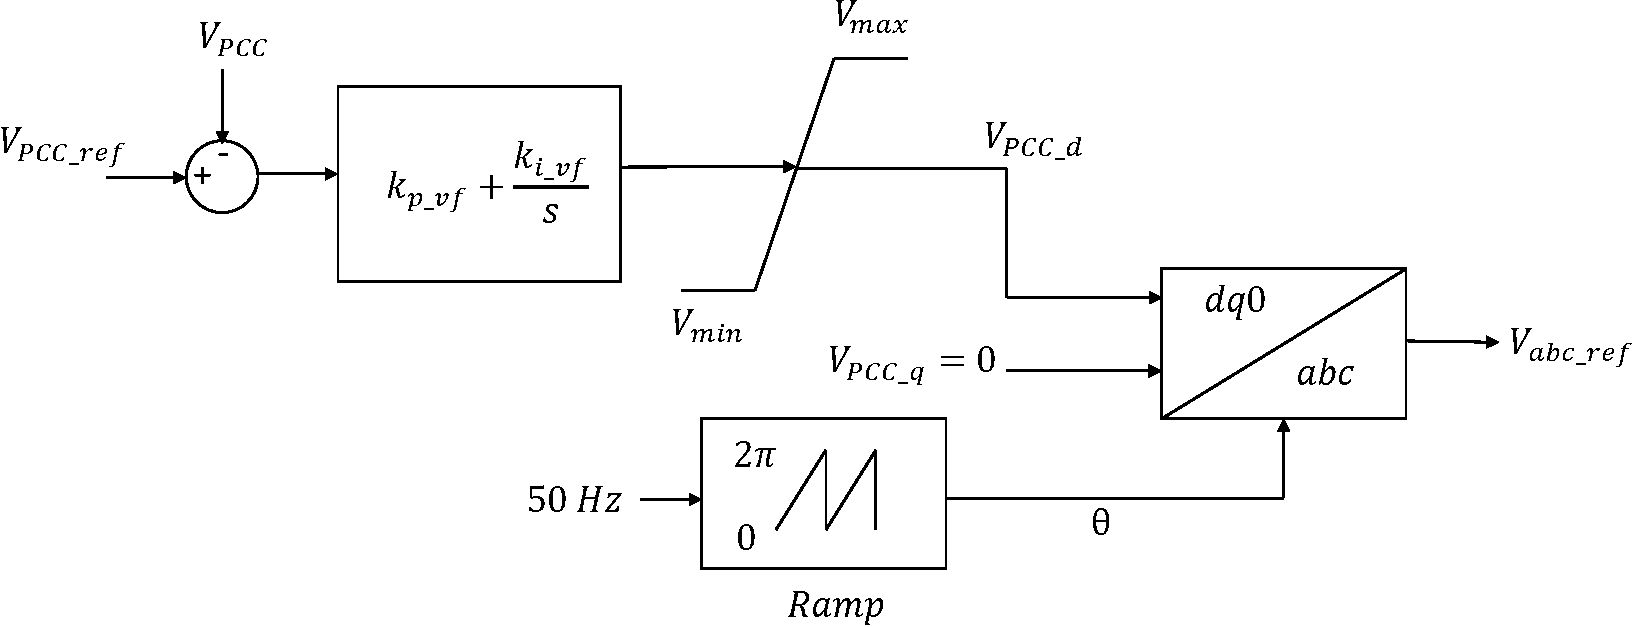
\includegraphics[height = 5cm,width = 12.5cm]{Diagrams/Chapter_4/U_F_control.pdf}
    \caption{U/F control mode in MMC-1 \cite{vrana2013cigre}}
    \label{fig:U_F_control}
\end{figure}

\begin{table}[H]
\centering
\begin{tabular}{|c|c|}
\hline
Parameter & Value \\ \hline
$k_{p\_vf}$     & 0.2 \\ \hline
$k_{i\_vf}$     & 30 \\ \hline
\end{tabular}
\caption{Parameters for PI gains in U/F control loop \cite{vrana2013cigre}}
\label{tab:U_F_para}
\end{table}

\subsection{Non- island mode control}
This mode of operation is based on the current vector control approach, which consists of the outer control loop and the inner control loop. The outer loop consists of the d and q axes loops. The d-axis loop can provide control of \gls{DC} voltage or active power and the q-axis loop can provide control of \gls{AC} voltage or reactive power. The outer control loop provides the respective current reference values as inputs for the inner current loops. The inner loop consists of \gls{PI} controllers for d and q axis separately and provides a decoupled control action. The output from the inner loop control is then translated back to the abc frame using dq0-abc frame transformation. \gls{MMC}-2 is configured with the current vector control in this work. 

Due to the common use of \gls{PI} controllers for control operation, it is convenient to translate from abc to rotating dq frame for analysis of three-phase circuits. Generally, for power system operation, while translating to dq frame, the voltage vector at \gls{PCC} is aligned along the d axis and the q axis component is aligned to zero as explained previously. This provides constant values for d and q components during steady-state, and it represents the three-phase components in two signal frame.

\gls{MMC}-2 identifies the frequency and phase angle at the point between both the interface transformers in \gls{MMC}-2 bus. The \gls{PLL} in \gls{MMC}-2 controls performs this task and synchronizes with the measured grid voltage. The phase angle is generated by the \gls{PLL} which is used to transform it from abc to dq frame. Such a type of control configures \gls{MMC}-2 to have a grid following action. The standard model available in \cite{vrana2013cigre} is modified and used for this work. The modification is brought out in the outer control loop and is explained in the following paragraph.    

\subsubsection{Modification in Outer Loop Control}
In order to simplify the system, the active power loop output variable which is the active power reference ($I_{d\_ref}$) is made to be controlled by the user using a slider ($ID\_ref\_control$) in Runtime file directly. This allows the user to control the amount of active power flowing through the \gls{MMC}-2 bus. The $I_{d\_ref}$ value is varied from 0 to a maximum of 0.4. There is no flow of power in \gls{MMC}-2 when $I_{d\_ref}$ = 0. The maximum power flow is achieved when $I_{d\_ref}$ = 0.4. %If $I_{d\_ref}$ is increased beyond 0.4, the transformer would be operated above 100\% of its rating and is not desirable. 

The RMS current ($I_{rms}$) is calculated at the breaker (CB-1a) and is compared with the maximum current ($I_{phase\_max}$) which is 10\% above the phase current as given in Equation \ref{i_phase_max_eq}. When the RMS current exceeds the maximum current, $I_{d\_ref}$ is set to zero for that duration. Once, $I_{rms}$ becomes less than $I_{phase\_max}$, the control is given back to the slider in Runtime module, as shown in Figure \ref{fig:Idref_control}. This allows power to flow in \gls{MMC}-2 after the breaker has been operated. The circuit breaker operation is explained in Section \ref{Fault logic and cb}.

\begin{equation}
    I_{phase} = \frac{S_{single\_phase}}{V_{LN}}
\end{equation}

\begin{equation}\label{i_phase_max_eq}
    I_{phase\_max} = 1.1 * I_{phase}
\end{equation}

\begin{figure}[H]
\centering
%\hspace*{-1.2cm}
    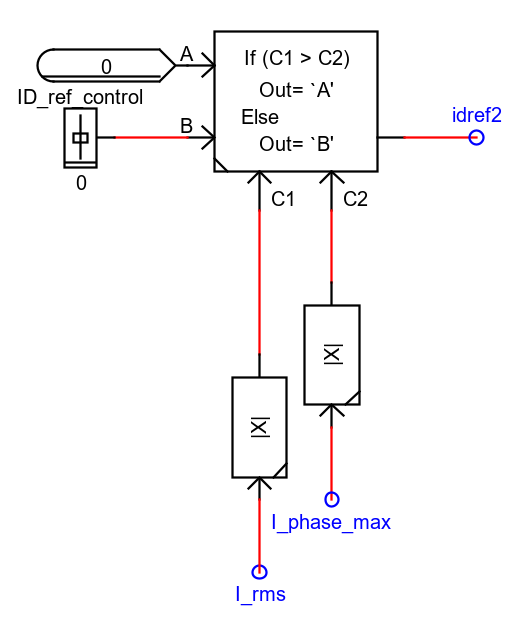
\includegraphics[height = 6cm,width = 5.5cm]{Diagrams/Chapter_4/Idref_control.PNG}
    \caption{$I_{d\_ref}$ control logic}
    \label{fig:Idref_control}
\end{figure}
